\documentclass[conference]{IEEEtran}
\IEEEoverridecommandlockouts
\pdfminorversion=7
\pdfcompresslevel=0
\pdfobjcompresslevel=0

\usepackage{cite}
\usepackage{amsmath,amssymb}
\let\proof\relax
\let\endproof\relax
\usepackage{amsthm}
\usepackage{graphicx}
\usepackage{booktabs}
\usepackage{array}
\usepackage{pifont}
\usepackage{xcolor}
\usepackage{colortbl}
\definecolor{bimrow}{HTML}{EAF2FC}
\usepackage{algorithm}
\usepackage[noend]{algpseudocode}
\usepackage{url}
\usepackage{microtype}
\usepackage[hidelinks]{hyperref}

% Artifact link, set in one place: the ISPA 2026 tag of the artifact repository.
\newcommand{\artifacturl}{https://github.com/assasin831/readseal-artifact/tree/ispa2026-r19}

\newcommand{\circled}[1]{\ding{\numexpr201+#1\relax}}   % black circled digits used in Fig. 1
\newcommand{\code}[1]{\texttt{#1}}
\newcommand{\hd}[1]{\textbf{\begin{tabular}[b]{@{}l@{}}#1\end{tabular}}}   % two-line table headers
\newcommand{\op}[1]{\textsc{#1}}                          % protocol transitions (Accept, Submit, ...)
\newcommand{\MiB}{\,MiB}
\newcommand{\ms}{\,ms}
\newcommand{\Hz}{\,Hz}
\newtheorem{proposition}{Proposition}

% Optional acknowledgment of the assistance used for this revision.
% Authors should review the acknowledgment against the submission requirements.
\newif\ifaidisclosure
\aidisclosurefalse
\setlength{\textfloatsep}{12pt plus 2pt minus 2pt}
\setlength{\dbltextfloatsep}{12pt plus 2pt minus 2pt}
\setlength{\floatsep}{10pt plus 2pt minus 2pt}

% Typographic conventions: italics mark a term at its definition (and math); bold run-in heads structure
% paragraphs; small caps name protocol transitions. Frame rates are in Hz; goodput is in results/s,
% where a result is one recipient's result bundle for one frame.

\begin{document}

\title{BIM and ReadSeal: Safe Early Reuse of\\ Shared GPU Buffers Across Processes}

\author{\IEEEauthorblockN{Xingbo Hui, Xuetao Jiang, Guodong Ye, Ruochen Shao, Tianyi Wang, Sicheng Wu, Rui Zhou\textsuperscript{*}, Qingguo Zhou\textsuperscript{*}}
\IEEEauthorblockA{School of Information Science and Engineering, Lanzhou University, Lanzhou, China\\
\textsuperscript{*}Co-corresponding authors: zr@lzu.edu.cn, zhouqg@lzu.edu.cn}}

\maketitle

\begin{abstract}
Processes in a perception pipeline often share one large GPU tensor instead of copying it for every recipient. When may the producer overwrite the shared buffer with the next frame? CUDA stream-only release waits only for submitted GPU work, so a component that has not started can read the wrong frame. Full retention waits for every result and can refuse new frames while the GPU is idle. Our key insight separates storage lifetime, ending at the last read, from frame identity, retained until every result is delivered. BEV-in-Memory (BIM) registers recipient processes when a frame is published; ReadSeal enrolls their reader components before GPU submission. ReadSeal analyzes storage sharing to locate each model's last source read and rejects execution that no longer matches its plan. Recipients finish on private intermediate results while the buffer holds the next frame. With four early-reading recipients on an A100, one shared buffer under BIM delivers 1.31--1.50$\times$ as many correct, timely results as full retention at 25--40\Hz. Mean and 95th-percentile latency increase by 8--11\ms{} and 15--19\ms, respectively, relative to one-buffer full retention. At 30\Hz, BIM also matches full retention with two buffers and a tuned limit on outstanding requests. Derived boundaries deliver as much as hand-placed ones and are rebuilt automatically after model changes. Ordered tests show that stream-only release lets a pending component read the next frame, whereas BIM with ReadSeal preserves the assigned frame.
\end{abstract}

\begin{IEEEkeywords}
GPU buffer reuse, zero-copy IPC, buffer lifetime, alias analysis, autonomous driving.
\end{IEEEkeywords}

% =====================================================================
\section{Introduction}
\label{sec:intro}

Consider a driving stack built on Autoware or another framework based on ROS~2, the Robot Operating System~\cite{autoware,ros2}. A camera--LiDAR fusion node publishes a bird's-eye-view (BEV) feature map, a top-down grid of features around the vehicle. Separate processes for 3D detection, tracking, motion planning, and data recording read it on their own schedules (Fig.~\ref{fig:overview}a). We call these processes \emph{recipients} and the components within them that access the map \emph{readers}. For example, BEVFusion feeds one BEV map to both a detection and a map-segmentation head~\cite{bevfusion}. Our evaluated map is a $1{\times}512{\times}180{\times}180$ fp32 tensor of 63.3\MiB~\cite{bevfusion}. Private copies for four recipients add 256\MiB{} of device memory (64\MiB{} each after allocator rounding), a cost that grows with the number of recipients and resident frames. The cost matters most on automotive systems-on-chip, whose GPU shares DRAM with the rest of the stack~\cite{cudategra}. Zero-copy middleware lets recipients map the sender's buffer~\cite{iceoryx,agnocast}, and recent ROS~2 facilities extend this to GPU memory~\cite{nitros,rosidlbuffer}. The producer must then decide when it may overwrite that buffer, which we call a \emph{slot}, with the next frame.

% ---------------------------------------------------------------------
\begin{figure*}[t]
\centering
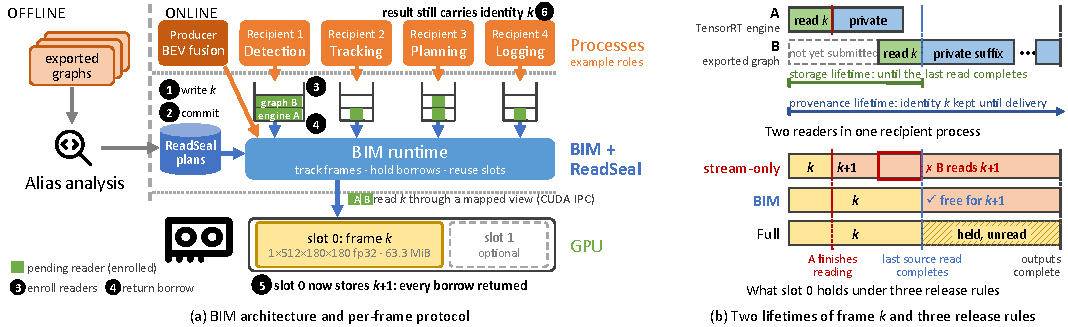
\includegraphics{figures/fig1_overview.pdf}
\caption{\textbf{BIM at a glance.} (a)~Offline, ReadSeal analyzes model graphs into plans. Online, the producer writes frame~$k$ and registers recipients at commit (\circled{1}, \circled{2}); ReadSeal enrolls their readers before submission (\circled{3}). Each recipient returns its borrow after its source reads complete (\circled{4}). Once all borrows return, the slot can hold $k{+}1$ (\circled{5}); results retain identity~$k$ (\circled{6}). (b)~Time runs left to right. Engine~A and graph~B belong to the last recipient holding a borrow. Stream-only permits overwrite before B reads; full retention waits for outputs; BIM with ReadSeal permits reuse after the last source read.}
\label{fig:overview}
\end{figure*}

Two common release rules leave a gap (Section~\ref{sec:motivation}). \emph{CUDA stream-only release}, shortened to stream-only in the figures, reuses the slot once all GPU work submitted so far has finished. A queued recipient that has not submitted its reads can then silently compute on the next frame. A detector would report objects seen in frame $k{+}1$ under the timestamp of frame $k$, and at 20\Hz{} a vehicle driving at 20\,m/s moves a full meter between the two. \emph{Full retention} holds the slot until every result is ready, as reference-counted zero-copy transports do when recipients keep their references until done~\cite{iceoryx,agnocast}. With a one-slot pool, a new frame is dropped while that slot is held. In our 20\Hz{} trace, the hold barely exceeds the frame period, so full retention drops every other frame and leaves the GPU idle between accepted frames (Fig.~\ref{fig:trace}).

\textbf{Key insight.} A shared tensor, the \emph{source}, has two lifetimes (Fig.~\ref{fig:overview}b). Its \emph{storage lifetime} ends when the last operation that reads it completes. Its \emph{provenance lifetime} preserves frame identity until every result is delivered, much as an essay cites a library book after the book is returned. In the TransFusion detection head, only the first of 287 operations reads our BEV map. The remaining operations use private intermediate results and can continue after the shared input is overwritten. Each recipient therefore needs its \emph{borrow}, permission to read the slot, only until its last source read completes.

Seen this way, full retention, copying, and early reuse are three choices of where a borrow ends: when the recipient's outputs are complete, when its private copy is complete, or when its last source read completes. All three must protect a recipient from before it starts reading.

Ending the borrow at the last read is safe only if the runtime can answer three questions. (1)~Which operation reads last? \emph{Views}, tensors that share the input's storage, extend its reads, so the \emph{read boundary} can come long after the source itself last appears (Fig.~\ref{fig:boundaries}). (2)~Who may still read? A reader that has not yet submitted GPU work leaves no event to wait on. (3)~Is the analyzed program the one that runs? A boundary derived for one model version can be wrong for the next.

We present BEV-in-Memory (BIM), a cross-process borrowing contract motivated by BEV sharing, and ReadSeal, the mechanism that answers these questions. BufferQueue and NvSciStream already let each consumer return a shared buffer independently~\cite{bufferqueue,nvscistream}. The application must decide when in each consumer's computation to return it and how to cover components that have not started reading. The producer knows only which processes receive a frame, so BIM registers each recipient's borrow at publication, before any recipient starts (Section~\ref{sec:bim}). Each process knows its reader components, so ReadSeal enrolls them before GPU submission, derives their last reads, and binds the plan to execution (Section~\ref{sec:readseal}).

Deriving the boundary matters because a hand-placed one can go stale or be wrong from the start. One added late read moves our detection head's boundary from the first operation to the second-to-last (Fig.~\ref{fig:boundaries}). A boundary after the first operation is correct for the head but wrong from the start for a ResNet-18 tail~\cite{resnet}. Its residual connection reads the source again at operation~12. A version check catches a stale boundary, not an incorrectly chosen current one. ReadSeal recomputes the boundary for each model version and rejects execution that no longer matches its plan. Our contributions are:
\begin{itemize}
\item \textbf{The two-lifetime view of a shared GPU tensor} (Sections~\ref{sec:intro}--\ref{sec:motivation}). Separating storage from provenance shows when a buffer can be reused while results keep their frame identity, and places full retention, copying, and early reuse on one axis.
\item \textbf{Checked release at a derived last read} (Sections~\ref{sec:bim}--\ref{sec:readseal}). BIM protects recipients from publication onward. ReadSeal enrolls their readers before submission, derives their last reads, and rejects execution that no longer matches its plan.
\item \textbf{An evaluation of the release choices} (Section~\ref{sec:eval}), comparing early reuse with full retention, extra slots, and copying under load, and testing the derived boundaries under ordered overwrites and model updates.
\end{itemize}

With early reads, one BIM slot matches two full-retention slots with a tuned request cap at 30\Hz, using one fewer 64\MiB{} buffer (Section~\ref{sec:eval-slots}). Derived boundaries deliver as much as hand-placed ones and follow model changes automatically. When reads occur late, copying can instead improve delivery at a memory and latency cost.

% =====================================================================
\section{Background and Motivation}
\label{sec:motivation}

\begin{figure}[t]
\centering
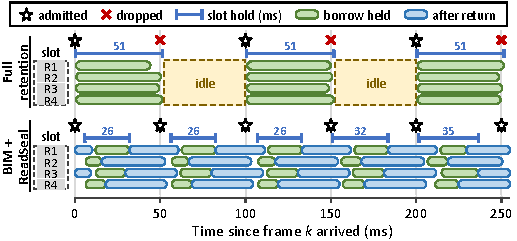
\includegraphics{figures/fig2_trace.pdf}
\caption{\textbf{Full retention refuses frames while the GPU idles.} Measured one-slot trace at 20\Hz{} (repetition~0); R1--R4 are the recipients, and labels give slot hold times in ms. Full's 51\ms{} hold just exceeds the 50\ms{} frame period, so it refuses every other frame even though the recipients sit idle; full retention is not work-conserving. Under BIM, each recipient's work after its borrow return overlaps the next frame.}
\label{fig:trace}
\end{figure}

\begin{figure}[t]
\centering
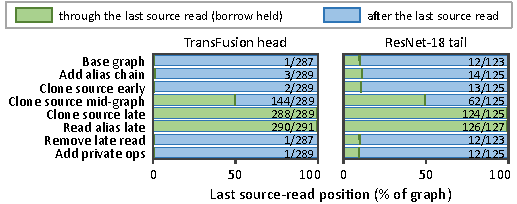
\includegraphics{figures/fig3_boundaries.pdf}
\caption{\textbf{Model edits move the last source read.} Each bar is a graph snapshot; green marks the operations through the last source read, during which the recipient holds its borrow. Each snapshot applies one edit to the base graph (Remove late read undoes Clone source late); labels give the last source-reading operation\,/\,total operations. Add alias chain inserts two storage-sharing views, which shift the operation indices but leave the runtime release point unchanged.}
\label{fig:boundaries}
\end{figure}

Each release rule below ends a recipient's borrow at a different point; Table~\ref{tab:options} compares them.

\textbf{GPU background.} A \emph{kernel} is a function executed on the GPU. A process places kernels in a \emph{stream}, which executes them in order, and continues without waiting. A read ends when its kernel completes. An \emph{event} marks a position in a stream and completes after the preceding work. PyTorch's \code{record\_stream} lets the caching allocator reuse a buffer only after the work already enqueued on the recorded streams has completed~\cite{recordstream}. CUDA inter-process communication (IPC) lets another process map the same device buffer and wait on shared events. But an event can only mark work that is already enqueued, so no process can wait on reads that another process has not yet submitted.

\textbf{Releasing too early fails silently.} The simplest case is a recipient still waiting in its queue. It has enqueued no GPU work, so a rule that waits only for submitted work, such as \code{record\_stream} or a read event, returns the slot once the other recipients' reads complete. The producer writes $k{+}1$, and the waiting recipient later computes a numerically valid result on it while its request still names $k$. No crash or error signals the failure, so a downstream planner has no reason to distrust the result. The same gap can open inside a recipient that combines a TensorRT engine with a framework graph. In our running example (Fig.~\ref{fig:overview}b), the two \emph{readers} are TensorRT engine~A, which signals an input-consumed event after reading its input~\cite{tensorrt}, and exported graph~B. An adapter forwards a view to the graph without reading the source itself. Once the engine's event completes, stream-only release returns the slot although the graph has not submitted its reads. Section~\ref{sec:eval-safety} tests this ordering. ROS~2's CUDA buffer backend exposes the same choice. A subscriber's read handle records a read event when it is destroyed, and the block is recycled once every handle is released~\cite{cudabackend}. Destroying the handle after the engine's read gives stream-only release; holding it until the outputs complete gives full retention.

\textbf{Holding the source through computation.} Full retention's hold refuses frames while the GPU idles (Fig.~\ref{fig:trace}). A second slot absorbs some of those arrivals but can admit more work than the GPU finishes before the deadline (Section~\ref{sec:eval-slots}).

\textbf{Copying the source.} A private copy lets a recipient compute after the shared slot is reused. The copy itself reads the source, however, so the slot must remain protected while a recipient is queued and until its copy completes. Our clone-on-accept policy uses BIM's recipient registration and ends each borrow at copy completion.

\textbf{Maintaining a read boundary.} A view can carry a source read into later operations (Fig.~\ref{fig:boundaries}), so a hand-placed boundary must be reviewed whenever the model changes. A stale boundary releases too early unless execution is guarded against the change.

\begin{table}[t]
\caption{Release options for four recipients ($K$: request cap). Extra memory counts source slots and input copies. $^\dagger$Manual uses an independent digest-checked runtime; Manual-checked uses BIM's runtime and checks. $^\ddagger$Misses readers that have not submitted work.}
\label{tab:options}
\centering
\footnotesize
\setlength{\tabcolsep}{1.8pt}
\begin{tabular}{@{}lllll@{}}
\toprule
\hd{Policy} & \hd{Extra\\memory} & \hd{Slot reusable\\after} & \hd{Read\\boundary} & \hd{Wrong\\frame?} \\
\midrule
Stream-only            & ---      & submitted reads & stream idle & possible$^\ddagger$ \\
Full retention         & ---      & all outputs     & ---         & no      \\
Full, 2 slots, $K{=}8$ & one slot & all outputs     & ---         & no      \\
Clone-on-accept        & 256\,MiB & all copies      & fixed       & no      \\
Manual$^\dagger$        & ---      & all last reads  & by hand     & no \\
Manual-checked$^\dagger$ & ---     & all last reads  & by hand     & no \\
\rowcolor{bimrow}
BIM + ReadSeal         & ---      & all last reads  & derived     & no \\
\bottomrule
\end{tabular}
\end{table}

% =====================================================================
\section{BIM: Frame Identity and Buffer Reuse}
\label{sec:bim}

BIM separates memory, frame identity, and permission to read. The producer has a pool of $N$ reusable GPU slots on one machine. It writes frame~$k$ into a slot and attaches an identity that every result from that frame carries. The same slot can later hold frame~$k{+}1$.

A recipient process holds one borrow until all its reader components, such as engine~A and graph~B, have finished reading the source, including readers still waiting to submit work.

\textbf{Descriptors and views.} Recipients receive small descriptors over a control plane such as ROS~2 and map the resident tensor, here through PyTorch's CUDA IPC support~\cite{torchmp}. A descriptor carries a frame identity (producer instance and sequence number), a storage locator, and an interpretation: element type, shape, strides, and a checked view range. The \emph{view} specifies which bytes a recipient may address and how to interpret them. BIM rejects stale identities and incompatible interpretations.

\textbf{Borrow bits and admission.} A process-shared lock protects slot reservation, the frame sequence, and borrow bits $b_{s,j}$ for each slot~$s$ and recipient~$j$. A set bit means that recipient~$j$ may still read slot~$s$. An arriving frame takes a slot whose bits are all clear; if none is free, the producer drops the frame instead of waiting. Once the frame is written, the producer \emph{commits} it by setting every recipient's bit before sending any descriptor. This protects recipients still waiting in their queues, before they can possibly read. Returning a borrow clears its bit; clearing the last bit permits reuse without freeing or unmapping the slot. If frame~$k$ is committed at time~$c_k$ and recipient~$j$ returns its borrow at time~$t_{j,k}$, the slot is held for $H_k$. With one slot, a frame arriving at time~$a$ is admitted only if
\begin{equation}
a\;\ge\; c_k+H_k, \qquad H_k=\max_j t_{j,k}-c_k. \label{eq:hold}
\end{equation}
Full retention sets $t_{j,k}$ to the time $j$'s outputs complete, and ReadSeal to the time $j$'s last source read completes (Section~\ref{sec:enroll}). This difference in hold time changes which new frames can enter. An optional cap~$K$ bounds outstanding recipient requests, counted from admission to receipt at the output sink. A frame must pass both admission gates: a free slot and room under the cap.

% =====================================================================
\section{ReadSeal: Checked Borrowing}
\label{sec:readseal}

ReadSeal prepares a \emph{plan} once per model version, then checks it each time a recipient processes a frame (Algorithm~\ref{alg:readseal}). The plan records where the graph stops reading shared storage, which components may read it, and which program version was analyzed. One execution of the plan is an \emph{invocation}. Its recipient returns the borrow when every planned source read has finished or was cancelled before starting.

\subsection{Deriving the Read Boundary}
\label{sec:derive}

\begin{algorithm}[t]
\caption{BIM's commit and ReadSeal's plan and invocation}
\label{alg:readseal}
\footnotesize
\begin{algorithmic}[1]
\Procedure{Publish}{frame $k$}\Comment{producer (BIM)}
\State \textbf{if} no slot is free or the request cap is reached, \textbf{drop} frame $k$
\State write $k$ into a free slot $s$; \emph{commit}: set $b_{s,j}$ for all $j$
\State send each recipient a descriptor of $(k,s)$
\EndProcedure
\Procedure{BuildPlan}{graph $G$, recipient $j$}\Comment{offline}
\State compute $Q_r$ by \eqref{eq:reads} and $\beta$ by \eqref{eq:boundary}
\State split $G$ at $\beta$; record readers $U_j$ and tokens $T$
\EndProcedure
\Procedure{Invoke}{plan, frame $k$}\Comment{recipient $j$}
\State check $T$; keep identity $k$ for every output
\State enroll every reader in $U_j$ before any of them submits GPU work
\State submit the stages in declared order, checking $T$ at each entry
\State \textbf{on} failed check: cancel unsubmitted reads, drain, publish nothing
\State \textbf{on} each completed or cancelled read: \textbf{if} \eqref{eq:return} holds, clear $b_{s,j}$
\State \textbf{on} completed outputs: publish them with identity $k$
\EndProcedure
\end{algorithmic}
\end{algorithm}

The analysis runs on each graph, a fixed-shape, functional directed acyclic graph (DAG) of operations. Of the two lifetimes, only storage needs analysis. Every result carries the frame identity attached at acceptance. Storage sharing propagates through views. A slice of the source is a view, so an operation on the slice still reads the source, whereas a convolution reads the source but writes fresh storage, so operations on its output do not. In our running example, the adapter only forwards a view; the graph receiving that view reads the source.

Formally, let $S(v)$ be the set of shared roots whose storage a value~$v$ may alias, with $S(r)=\{r\}$ for the source~$r$. For an operation~$o$ with inputs $v_h$ and output $v_o$, let $\mathcal{A}_o$ index the inputs the output may alias and $\mathcal{R}_o$ the inputs $o$ reads. Then
\begin{equation}
\begin{aligned}
S(v_o)&=\textstyle\bigcup_{h\in \mathcal{A}_o} S(v_h),\\
Q_r&=\{\, o : \exists\, h\in \mathcal{R}_o,\; r\in S(v_h) \,\},
\end{aligned}\label{eq:reads}
\end{equation}
where $Q_r$ is the set of operations that may read the source. With the operations numbered $o_1,\dots,o_n$ in execution order, the read boundary is the position of the last one in $Q_r$,
\begin{equation}
\beta=\max\bigl(\{0\}\cup\{\, i : o_i\in Q_r \,\}\bigr), \label{eq:boundary}
\end{equation}
so the \emph{source-reading prefix}, $o_1,\dots,o_\beta$, includes all source reads. If $Q_r=\varnothing$, then $\beta=0$ and the prefix is empty. The \emph{private suffix}, $o_{\beta+1},\dots,o_n$, computes the remaining results using private intermediate storage. Fig.~\ref{fig:boundaries} labels each graph snapshot with $\beta/n$; the base head has $\beta=1$ and $n=287$.

Operator summaries cover 42 reviewed operator variants in ATen, PyTorch's operator library, plus fixed-index tuple selection. Each summary counts every operand as read and treats an output as sharing storage whenever the operator's declared signature permits aliasing with an input. Plan construction rejects unsupported mutation, opaque callbacks, and source views that escape the graph. The implementation compiles the prefix and suffix into separate executable stages. A CUDA event after the prefix then marks the end of its source reads.

\subsection{Enrolling Readers Before Submission}
\label{sec:enroll}

Registration covers recipient processes and their reader components (Section~\ref{sec:bim}). BIM sets each recipient's borrow bit at commit. At frame acceptance, ReadSeal registers, or \emph{enrolls}, all readers in that recipient before any submits GPU work. Each reader~$u$ marks its last source read with a completion event: A's input-consumed event or the event after B's prefix. Let $U_j$ be the readers of recipient~$j$. Then $j$ returns its borrow for frame~$k$ at the first moment when
\begin{equation}
\forall u\in U_j:\quad \mathit{done}_u \lor \mathit{cancelled}_u, \label{eq:return}
\end{equation}
where $\mathit{done}_u$ holds once $u$'s completion event has completed and $\mathit{cancelled}_u$ once $u$ has been cancelled before submission. Every enrolled reader participates in this condition. When A's event completes, B's read is still pending, so the bit stays set even though B has enqueued no GPU work. Returning the borrow clears $j$'s bit. Once all recipients have returned their borrows, the producer can write the next frame while $j$'s private suffix continues computing results labeled~$k$.

% Fig. 5 is defined here, inside Section IV (page 4), so that it floats to the top of the page where Section V starts.
% ---------------------------------------------------------------------
\begin{figure*}[t]
\centering
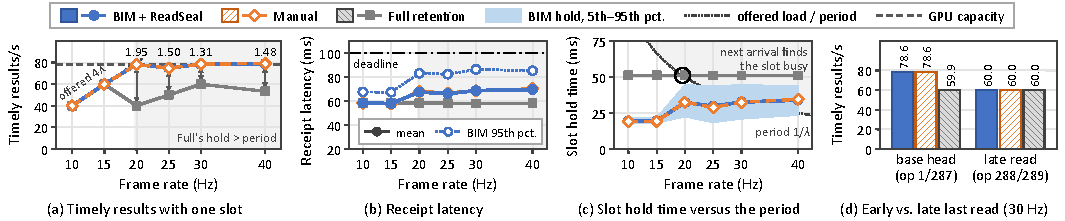
\includegraphics{figures/fig5_delivery.pdf}
\caption{\textbf{Early reuse raises one-slot delivery under load, with a latency cost.} One slot, no pipeline-wide cap~$K$; six runs per condition and policy. Each input frame offers four recipient results; results/s counts individual results. (a)~Labels give BIM/Full ratios. (b)~Mean receipt latency; BIM's 95th percentile is computed per run and averaged. (c)~Mean hold and BIM's 5th--95th percentile; shading marks where Full's hold exceeds the frame period. (d)~Moving the last read to the graph's end removes the gain.}
\label{fig:delivery}
\end{figure*}

\subsection{Binding Plans to Execution}
\label{sec:bind}

At construction, ReadSeal captures the functions to run and copies the model's parameters and buffers once into plan-owned storage, so later edits by the caller cannot change a plan in use. The manual implementation does the same.

ReadSeal records \emph{binding tokens}~$T$, identifiers and metadata for code and globals, model storage and version, input layout, and compiled stages. At acceptance and each stage entry it compares them with the values for the execution about to run, $\hat T$, and proceeds only if $\hat T=T$. A failed check cancels unsubmitted reads, drains started work, and publishes nothing. The application supplies the exported graph, each native engine's last-input-read event, and the component and output dependencies. New operators require reviewed summaries.

\subsection{Correctness Conditions}
\label{sec:correctness}

The analysis must include every operation that can read the source. It assumes that operator summaries conservatively describe reads and storage sharing, kernels obey those summaries, and the graph executes in the analyzed order.

\begin{proposition}
Under these assumptions, $Q_r$ in Eq.~\eqref{eq:reads} contains every operation that can read the shared source. No operation after the derived boundary $\beta$ reads that source.
\end{proposition}

\begin{proof}[Proof sketch]
Initially $S(r)=\{r\}$. At each operation, the union in Eq.~\eqref{eq:reads} preserves the shared roots of every input that its output may alias. Induction over graph order therefore includes every source alias in the corresponding $S(v)$. The read rule places every operation consuming such storage in $Q_r$; by Eq.~\eqref{eq:boundary}, none has an index greater than $\beta$.
\end{proof}

For the runtime, each reader's completion event must occur after its source reads, mappings must remain valid, and identities must remain unique while referenced. Algorithm~\ref{alg:readseal} registers every reader before submission, checks the plan at execution, and returns a borrow only when Eq.~\eqref{eq:return} holds. BIM permits overwrite after all recipient bits clear. Together, these steps preserve the source until every reader finishes, while results keep the identity captured at acceptance.

% =====================================================================
\section{Evaluation}
\label{sec:eval}

The evaluation asks when early reuse improves delivery, how slots and request caps interact, whether jitter or mixed recipients change the result, whether reuse stays safe as models change, and what the checks cost.

% The slots figure is defined at the start of Section V so that it floats to the page after the delivery figure.
\begin{figure*}[t]
\centering
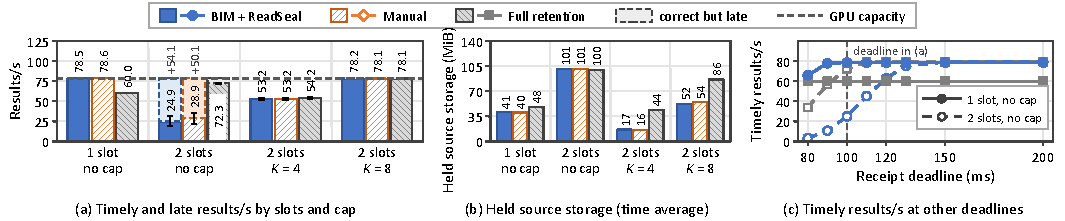
\includegraphics{figures/fig6_slots.pdf}
\caption{\textbf{One BIM slot matches full retention with two slots and a request cap} (30\Hz; six runs per condition and policy). $K$ counts outstanding recipient requests; eight requests are two full groups of four. (a)~Solid: timely results; dashed: correct but late; whiskers: 95\% intervals. (b)~Time-averaged source storage held by unreturned borrows, not allocated memory. Device peaks are 5,078\MiB{} with one slot and 5,142\MiB{} with two for every policy. (c)~BIM and Full re-scored at different deadlines using the same runs.}
\label{fig:slots}
\end{figure*}





\subsection{Setup}
\label{sec:eval-setup}

\textbf{Scope and platform.} We evaluate cross-process reuse of saved BEV features on one NVIDIA A100 PCIe 40\,GB GPU. The producer, four recipients, and output sink communicate through multiprocessing queues and share storage and events through CUDA IPC. Saved features isolate reuse and admission from feature extraction; the setup does not run ROS~2, the BEV front end, or an embedded driving stack. The runtime uses PyTorch 2.1.2, CUDA 12.1, and TensorRT 10.3. Without NVIDIA's Multi-Process Service (MPS), recipient kernels take turns on the GPU. Records, validators, campaign details, and analysis scripts are public.\footnote{\url{\artifacturl}.}

\textbf{Workload.} The exported graph (B) is BEVFusion's functional TransFusion head~\cite{bevfusion,transfusion}, with 287 operations. The producer publishes precomputed 63.3\MiB{} feature maps from three fixed nuScenes-mini frames~\cite{nuscenes}. The native engine (A) runs the head's shared convolution, ReLU, and global average pooling in TensorRT; an adapter forwards a view to the graph. This controlled composition gives each recipient two readers of the same source, each with its own completion event. Four recipients run identical compositions in the rate and slot sweeps; Section~\ref{sec:eval-mixed} varies their components. A pretrained ResNet-18 tail~\cite{resnet}, made of the residual stages and classifier with saved stem activations as the shared source, serves in the correctness, model-change, and cost tests.

\textbf{Policies.} All policies share the pool, workloads, queues, and admission settings. BIM uses ReadSeal, and \emph{Full} retains the source until its outputs complete. Two hand-placed baselines come from different campaigns. \emph{Manual}, used in the earlier rate and slot campaigns, is a separately implemented runtime that registers both readers and checks code and model digests, so it tests early reuse independently of our runtime. \emph{Manual-checked}, used in the later jitter and mixed-recipient campaign, shares BIM's runtime and binding checks and differs only in where the boundary comes from, which isolates automatic placement. \emph{Clone-on-accept} gives each recipient a private input copy when it accepts a request.

\textbf{Metrics.} The producer schedules frames at rate~$\lambda$, in Hz. Each frame should yield four \emph{results}, one output bundle per recipient, so the offered load is $4\lambda$ results/s. A result is \emph{timely} if it passes source-identity and reference-output checks and reaches the output sink, after device-to-host transfer and IPC, within 100\ms{} of the frame's planned arrival. The 100\ms{} budget is a common benchmark threshold rather than a vehicle requirement, so we also re-score the slot runs at 80--200\ms. \emph{Receipt latency} runs from planned arrival to sink receipt; \emph{slot hold time} runs from commit to the last borrow return. The complete-frame timely fraction (Section~\ref{sec:eval-mixed}) counts a frame only if all four intended results are correct and timely, and its denominator includes refused and partially admitted frames.

\textbf{Queue settings.} The rate and slot sweeps permit at most two pending requests and four in flight per recipient. Optional cap~$K$ limits outstanding recipient requests across the pipeline; $K{=}8$ accommodates two full groups of four requests. \emph{No pipeline-wide cap} leaves the per-recipient queue limits in place. Because the producer drops frames rather than blocking, every policy sees the same offered load.

\textbf{Statistics.} Rate and slot runs have 2\,s of warm-up, 12\,s of measured arrivals, and a complete drain. Condition and method order are randomized, with six paired repetitions per condition; brackets give pointwise 95\% intervals from 20,000 paired whole-run bootstrap draws. The two campaigns in Section~\ref{sec:eval-mixed} use queues of eight, 10\,s of warm-up, and 30\,s of measurement, with six paired runs and pointwise 95\% $t$ intervals. Campaigns are analyzed separately. Latency summaries describe individual recipient results in the rate sweep (mean and per-run 95th percentile) and complete correct frames in the mixed-recipient study (per-run 99th percentile).

\subsection{Early Reuse Raises Delivery Under Load}
\label{sec:eval-delivery}

Early reuse improves delivery once the frame period drops below full retention's hold time (Fig.~\ref{fig:delivery}a). Both policies keep up at 10 and 15\Hz. At 20\Hz, where Full accepts only every other frame, BIM delivers 1.95$\times$ as many timely results as Full. At 25--40\Hz, the BIM/Full ratio is 1.31--1.50$\times$. BIM stays within 0.2 results/s of Manual at every rate.

\textbf{Slot hold time.} Full holds the slot for about 51\ms, nearly the entire computation of the four recipients. BIM cuts the hold to 30--34\ms{} (Fig.~\ref{fig:delivery}c). Each head reads the source in its first operation, but the last recipient must wait for its turn on the shared GPU. Earlier return admits the next frame during private computation, filling the idle gaps of Fig.~\ref{fig:trace}. At 25\Hz, BIM's timely delivery dips to 75.0 results/s in all six runs, versus means of 78.3--79.0 at 20, 30, and 40\Hz. The 40\ms{} arrival period interacts with slot availability: a refused arrival is not retried, so the next admission opportunity is a full period later.

\textbf{Receipt latency.} The additional admitted work queues behind other recipients on the GPU. At 20--40\Hz, BIM's mean latency is 8--11\ms{} higher than Full's and its per-run 95th percentile 15--19\ms{} higher (Fig.~\ref{fig:delivery}b). The delivery lead at 30\Hz{} holds across 100--200\ms{} deadlines and narrows at 80\ms, where more of this queued work arrives late (Fig.~\ref{fig:slots}c).

\textbf{Late source reads.}\label{sec:eval-late} Moving the last source read to operation 288 of 289 leaves almost no private computation to overlap (Fig.~\ref{fig:boundaries}'s late clone). BIM's hold then reaches Full's, and all three policies deliver 60.0 results/s at 30\Hz{} (Fig.~\ref{fig:delivery}d). The gain comes from overlapping the private suffix with the next frame.

\subsection{One Slot Matches Two, and Two Need a Cap}
\label{sec:eval-slots}

A second slot is the usual remedy for full retention's refusals (Fig.~\ref{fig:slots}a). At 30\Hz, two-slot Full with $K{=}8$ delivers 78.1 results/s, matching one-slot BIM's 78.5, so BIM reaches the same delivery with one fewer source buffer. In this pipeline that buffer is 64\MiB{} of a device peak of roughly 5\,GiB. The second slot also makes the cap decisive: $K{=}4$ holds every policy to 53--54 results/s, and no cap lets work miss the deadline.

\textbf{Queueing with two slots.} With one slot, the hold time in Eq.~\eqref{eq:hold} paces BIM's admissions. A second slot removes that pacing and lets requests queue before the GPU can start them. Without a pipeline-wide cap, two-slot BIM delivers only 24.9 timely results/s against Full's 72.3, and another 54.1 results/s arrive correct but late. Full's longer hold still throttles its arrivals. Manual shows the same drop, and a looser deadline recovers the delayed results (Fig.~\ref{fig:slots}c).

\textbf{Request cap.} At $K{=}8$, all three policies reach similar delivery across the two-slot rate sweep. BIM still returns borrows sooner, so the time-averaged source storage held by outstanding borrows falls from 86.4\MiB{} under Full to 52.3\MiB{} (Fig.~\ref{fig:slots}b). The metric counts locked storage rather than allocation; returning a borrow makes a slot reusable without freeing it, so the device peak is unchanged.

\subsection{Jitter, Mixed Recipients, and Copying}
\label{sec:eval-mixed}

\begin{figure}[t]
\centering
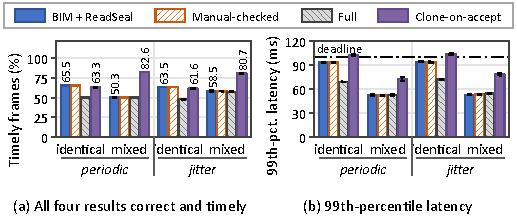
\includegraphics{figures/fig7_mixed.pdf}
\caption{\textbf{Complete-frame delivery and tail latency with jitter and mixed recipients} (30\Hz, one slot, no pipeline-wide cap; 6 runs per bar; whiskers: 95\% $t$ intervals). (a)~Share of the 900 scheduled frames per run whose four results are all correct and timely; (b)~per-run 99th-percentile latency of frames whose four results are all correct. \emph{Identical}: four copies of the composition; \emph{mixed}: four component profiles, one reading late.}
\label{fig:mixed}
\end{figure}

This study asks whether every intended recipient finishes on time, using the complete-frame metric (Fig.~\ref{fig:mixed}). At 30\Hz{} with one slot and no pipeline-wide cap, arrivals are periodic or displaced by up to 0.8 of a period (\emph{jitter}). Recipients are either \emph{identical} copies of the composition or \emph{mixed}: the native engine alone, the exported head alone, their composition, and a composition that reads the source late.

\textbf{Arrival pattern and recipient mix.} With identical recipients, BIM completes 65.5\% of frames on time under periodic arrivals and 63.5\% with jitter, about 15.5 percentage points above Full in both cases. With mixed recipients, the recipient containing a late reader retains its borrow longer, and BIM stays less than one point above Full (Fig.~\ref{fig:mixed}a). Jitter raises mixed-recipient delivery from 50.3\% to 58.5\% for BIM and from 50.0\% to 57.5\% for Full. This is consistent with irregular arrival gaps allowing more frames past a hold that otherwise refuses every second periodic arrival.

\textbf{Input copying.} Clone-on-accept releases the shared input after copying, even when computation will read the private copy much later. With mixed recipients it completes 22--32 percentage points more frames on time than BIM, at a 256\MiB{} higher sampled device peak and 20--25\ms{} more 99th-percentile latency. With identical early-reading recipients it completes about two points fewer.

A separate 168-run study counts individual recipient results. With early readers, BIM delivers 0.4--0.9 results/s more than cloning at 20, 30, and 40\Hz; cloning leads by 2.75 [2.47, 3.03] at 25\Hz, where BIM shows its admission dip. When all readers read late at 30\Hz, cloning delivers 76.4 results/s against 60.0, a paired gain of 16.39 [16.06, 16.72], but raises the mean per-run 99th-percentile latency from 68.7 to 101.1\ms{} and worsens freshness. Its sampled device peak is 5,334\MiB, against BIM's 5,078\MiB.

\textbf{Hand-placed comparison.} Across this study, including its 12 all-late runs, Manual-checked stays within 0.13 percentage points of BIM. With the runtime and checks held fixed, deriving the boundary automatically costs nothing in delivery.

\subsection{Safety Across Reordering and Model Changes}
\label{sec:eval-safety}

\textbf{Future readers.} In six controlled ordered tests, engine~A's input-consumed event completes before graph~B submits its reads. Under stream-only release, the graph's outputs matched the replacement frame in every test, because recording stream use cannot cover reads that have not been submitted~\cite{recordstream}. Under BIM and Manual, they matched the admitted frame. Under load, all 109,592 results delivered by BIM, Manual, and Full in the 144 rate and late-read runs carried their admitted identity and matched reference outputs.

\textbf{Boundaries under model change.} Regenerated boundaries kept every output exact. Across eight snapshots per model, three inputs, and two methods, all 96 ordered-overwrite cases (540 output tensors) matched unsplit references, and binding validation rejected all 22 attempted substitutions of plan, code, globals, model state, or input before the affected stage ran.

\textbf{Boundary maintenance.} We replay 16 controlled transitions: 14 graph edits, one batch-normalization folding, and a public ResNet-18 to ResNet-50 substitution. The runtime release point moves in 13 of them; folding keeps the head's first source read, and the two alias-chain edits only renumber operations (Fig.~\ref{fig:boundaries}). Binding checks reject all 16 outdated hand-placed plans (the model substitution is checked on the CPU), so a manual deployment waits until someone refreshes its plan. ReadSeal rebuilds the updated plans in 0.08--0.21\,s on the CPU without source-reader or boundary annotations. The mixed-recipient tests show the same pattern. After a late read was added, Manual-checked's old boundary failed its check until the boundary was moved, and all 24 update cases then gave exact outputs.

\subsection{Execution Cost and Coverage}
\label{sec:eval-cost}

An isolated-process test times recipient acceptance to output dispatch (8 process repetitions of 50 randomized invocations per method; three inputs; base and late variants of both models). ReadSeal's checks add 0.8--0.9\ms{} per invocation, mostly at acceptance and stage submission. That is 8\% over Manual for the base head (11.8\ms{} against 10.9\ms) and 22--23\% for the lighter ResNet tail. In the pipelines above the cost overlaps GPU work, and even at 10 and 15\Hz{} BIM's mean receipt latency is within 0.4\ms{} of Manual's. A static survey of 14 torchvision tails accepts nine, with boundaries in their first 1--12 operations, and rejects five for unsupported operators.

% =====================================================================
\section{Discussion}
\label{sec:discussion}

\textbf{Why derive the boundary?} Hand-placed boundaries delivered as much as derived ones in every campaign, so ReadSeal's value is correctness as models change. Binding checks reject a plan built for other code, weights, or inputs, but they cannot tell whether a current boundary was right to begin with, such as one placed after the ResNet tail's first operation or one that misses a late read through a view (Fig.~\ref{fig:boundaries}). ReadSeal finds both in the graph. It still relies on reviewed operator summaries, native input-consumed events, and declared component dependencies; missing summaries caused all five survey rejections.

\textbf{Choosing a release policy.} The last source read and available memory determine where a borrow should end. Early reuse suits early readers when per-recipient copies are too costly. Late readers leave little private work to overlap; copying can then improve delivery at a memory and tail-latency cost (Section~\ref{sec:eval-mixed}). With spare memory and a tunable cap, extra slots or copies are simpler. Release and admission must also be considered together. In our one-slot pipeline, the hold time paced admissions so every admitted result arrived on time; with two slots, a request cap was needed.

\textbf{Portability.} BIM needs cross-process storage mapping and completion events that cover each reader's source access. ROS~2's CUDA buffer read handles~\cite{cudabackend} and NvSciStream's per-consumer packet release~\cite{nvscistream} are natural integration points. A port would create each consumer's hold before the frame is published, release it on ReadSeal's completion event, and validate the platform's ordering guarantees.

\textbf{Deployment.} The prototype runs declared topologies with single-stream stages, and a topology change requires a new plan. A crashed recipient leaves its borrow outstanding and blocks slot reuse, so recovery must confirm that the recipient's GPU work has stopped before its borrow is removed.

% =====================================================================
\section{Related Work}
\label{sec:related}

\textbf{Zero-copy robotics middleware.} iceoryx and Agnocast give ROS~2 subscribers direct access to publisher-owned shared memory~\cite{iceoryx,agnocast}. NITROS's composable graphs share GPU data within one process~\cite{nitros}, while ROS~2's \code{rosidl::Buffer} supports cross-process sharing through CUDA IPC~\cite{rosidlbuffer}. Sharing a buffer still leaves the application to determine when it may be reused while a recipient has yet to read it.

\textbf{Release fences.} Android's BufferQueue lets a consumer release a pooled buffer with a fence while still reading it~\cite{bufferqueue}. NvSciStream returns a multicast packet to its pool once every consumer has released it~\cite{nvscistream}. BIM's borrow bits follow this per-consumer protocol. ReadSeal adds the fence's position, deriving each graph reader's last source read from its model.

\textbf{Asynchronous buffer protocols.} Simpson's four-slot mechanism separates concurrent reads and writes across buffers. Kopetz and Reisinger's non-blocking write (NBW) protocol detects overlapping writes and provides a multibuffer variant~\cite{simpson,nbw,rushbyfour}. Cyclical asynchronous buffers let readers acquire the latest complete value without blocking the writer~\cite{buttazzocab}. BIM instead preserves the particular frame already assigned to each recipient, including while its GPU reads are unsubmitted. ReadSeal supplies the model-derived point at which that borrow ends.

\textbf{Last use and safe reclamation.} Compilers and runtimes reuse a buffer after its last use, as in TVM's static memory planning~\cite{tvm}, and Rust's non-lexical lifetimes end a borrow there~\cite{nll}; both see every use in one program, in program order. % Dropped automatically when the acknowledgment is enabled, so the paper stays within eight pages.
\ifaidisclosure\else Task runtimes such as Legion and StarPU know future accesses because tasks declare their data when submitted~\cite{legion,starpu}. \fi
BIM's recipients are separate processes that declare nothing to the producer. Safe memory reclamation, such as read-copy-update (RCU) grace periods~\cite{rcu}, reuses memory once no reader can hold it, but protects only readers that have announced themselves. In RCU terms, BIM's commit opens every recipient's read-side section on its behalf, and ReadSeal closes it at the derived last read. ReadSeal's bindings, like PyTorch~2's guards~\cite{pytorch2}, reject execution whose assumptions changed.

% =====================================================================
\section{Conclusion}

Shared storage can be reused before results are ready if every pending reader is protected and its last source read is known. BIM registers recipient processes at publication; ReadSeal enrolls their readers, derives graph read boundaries, and checks execution against the analyzed plans. In our A100 pipeline, one BIM slot delivered 1.31--1.50$\times$ as many timely results as one-slot full retention at 25--40\Hz, with 8--11\ms{} more mean latency. At 30\Hz, it matched two full-retention slots with a tuned request cap. Derived boundaries matched hand-placed delivery and followed every replayed model edit. Among the surveyed torchvision tails, all nine accepted graphs stopped reading their inputs within 12 operations. Late readers instead favor copying when memory allows. Next steps are ROS~2 and NvSciStream integration, embedded-CPU measurements, concurrent recipients, and selective copying for late readers.

\ifaidisclosure
\section*{Acknowledgment}
OpenAI Codex and Anthropic's Claude were used to edit and restructure the text throughout the paper, update figure labels, and cross-check reported numbers against the experimental records. The experiments, data, and figure content are the authors' own.
\fi

\bibliographystyle{IEEEtran}
% Both columns of the last page fill without \IEEEtriggeratref.
\bibliography{refs}

\end{document}
